\lab{Application}{Depth and Breadth-First Searching with Kevin Bacon}{Depth and Breadth-First Searching with Kevin Bacon}
\label{lab:SixDegreesKevinBacon}

\objective{This section teaches about searching graphs and uses the parlor game ``the Six Degrees of Kevin Bacon'' as an application to graphs.}

\section*{Graphs}
\label{Graphs_section}
We commonly use graphs to represent the relationships between objects in a set. A graph is
represented by a set of nodes (objects) and a set of edges (relationships) where each edge
connects exactly two nodes. We would indicate an edge from node $x$ to node $y$ by $(x, y)$
and an edge from $y$ to $x$ by $(y, x)$. If \emph{all} of the edges within a graph are bidirectional
between their connecting nodes, the graph is said to be \emph{undirected}. If, however, the directions
of a graph's edges are specified, then the graph is said to be \emph{directed}. In this lab we will largely work
with undirected graphs.

There are two different data structures that can be used to represent graphs: adjacency matrices and adjacency lists.
Each data structure has its own advantages and disadvantages; the structure we use depends on the type of problem we are solving.

\begin{figure}[h]
\centering
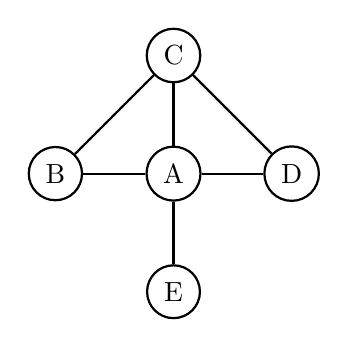
\begin{tikzpicture}[auto,node distance=1.5cm,
 thick,main node/.style={circle,draw}]

  \node[main node] (1) {A};
  \node[main node] (2) [left of=1] {B};
  \node[main node] (3) [above of=1] {C};
  \node[main node] (4) [right of=1] {D};
  \node[main node] (5) [below of=1] {E};

  \path[every node/.style={font=\sffamily\small}]
     (1) edge node [] {} (4)
     	  edge node [] {} (3)
     	  edge node [] {} (5)
     (2) edge node [] {} (1)
     	  edge node []{}(3)
     (3) edge node []{}(4);
\end{tikzpicture}
\caption{Example Graph 1}
\label{Adjacency}
\end{figure}


\subsection*{Adjacency Matrices}
An adjacency matrix is two dimensional matrix that is used to represent a graph. To construct an adjacency matrix, we order
the nodes of the graph and allow each node to correspond to one column and one
row of the matrix. Therefore, if we have $n$ nodes, we use an $n \times n$ matrix to
represent the edges between the nodes. In an unweighted graph (a graph where all the edges have the same value), we indicate an
edge using either a $0$ or a $1$.
Consider Example Graph 1 in Figure \ref{Adjacency}. Because a bidirectional edge exists between A and D, for example, we put a $1$ in the $(3, 0)$ position and
in the $(0, 3)$ position. Since no edge exists between A and C, we put a $0$ in
the $(2, 0)$ position and $(0, 2)$ position. We can represent the adjacency matrix for this graph as follows:

\[
\bordermatrix{\hspace{.4cm}&A&B&C&D&E\cr
                A&0 & 1 & 0 & 1 & 1\cr
                B& 1 & 0 & 1 & 0 & 0\cr
                C& 0 & 1 & 0 & 1 & 0\cr
                D& 1 & 0 & 1 & 0 & 0\cr
                E& 1 & 0 & 0 & 0 & 0}\]
Note that because this graph is undirected, its adjacency matrix is symmetric.

\subsection*{Adjacency Lists}
An adjacency list links each node of the graph to a list of its corresponding neighbors, the nodes to which it is connected by an edge.
There are many ways to index the nodes so we can easily access their adjacent neighbors, but, in Python, one of the most straightforward ways is to use a simple dictionary.
We could represent Graph 1 using the following code:
\begin{lstlisting}
AList = {'A': ['B', 'D', 'E'], 'B': ['A', 'C'], 'C': ['B', 'D'], 'D': ['A', 'C'], 'E': ['A']}
# To obtain a list of the nodes adjacent to A, simply access the
# dictionary at the key 'A'.
print Alist['A']
# You should obtain the following output:
['B', 'D', 'E']
\end{lstlisting}
We can retrieve the neighbors of any node of the graph in constant time.
This makes algorithms that operate locally on the graph highly efficient.

\section*{Searching Graphs}
There are two common ways to search a graph, both of which present different advantages depending on the purpose of the search.
One method is called a depth-first search (DFS).  It is designed to search the deepest levels of a graph first.
The other method is called a breadth-first search (BFS).  A BFS searches a graph one level at a time until it finds a solution.

\begin{figure}[h]
\centering
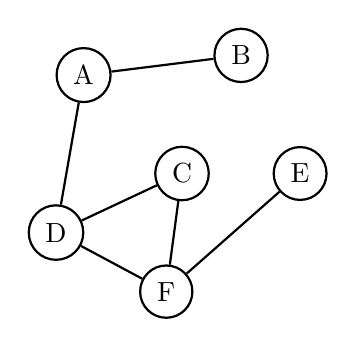
\begin{tikzpicture}[auto,node distance=1.5cm,
 thick,main node/.style={circle,draw}]
\centering
  \node[main node](1) at (-1.25,1.25) {A};
  \node[main node](2) at (.75,1.5)  {B};
  \node[main node](3) at (0,0) {C};
  \node[main node](4) at (-1.6,-.75) {D};
  \node[main node](5) at (1.5,0)  {E};
  \node[main node](6) at (-.2,-1.5)  {F};

  \path[every node/.style={font=\sffamily\small}]
  	(2) edge node[]{}(1)
  	(4) edge node[]{}(1)
  	     edge node[]{}(3)
  	     edge node[]{}(6)
	(6) edge node[]{}(3)
	     edge node[]{}(5);
\end{tikzpicture}
\caption{Example Graph 2}
\label{bfs_dfs}
\end{figure}

Using Graph 2 in Figure \ref{bfs_dfs}, we will walk through two examples of a depth-first search.
In these examples, when a node has multiple branches originating from it,
we will visit the latest (greater) letter in the alphabet first.
The node at which the algorithm begins is called the ``root node''.
First, we will use D as our root node and E as our target node.
Starting with D, we look at D's greatest neighbor, F, then at F's greatest
neighbor, E. Since E is our target, the algorithm ends.

Second, we start with A and search for B.
We visit node A, then D, then F, and finally E.
At this point, we have gone to the deepest level possible without finding our target, B.
We must back up and try another branch of nodes;
the algorithm backtracks from E to F to try another route.
Here, it is very important that we mark those nodes we have already visited,
otherwise the algorithm would infinitely loop around the latter portion of
the graph without reaching our target, B. Since we have marked D as previously visited, we visit F's final neighbor, C.
We return to node F. Since we have already
searched all possible nodes adjacent to F, we backtrack, again, to D. Because we have
exhausted all sub-branches originating from D, we travel back to A and try
any unexplored branches there. Finally, we find B and the algorithm ends.

Let's try the same two searches using a breadth-first search. While exploring our branches this time, however,
we will visit the earliest (lesser) letter in the alphabet first. In this first search, we again use D as our root node and
E as our target node.
We start by searching for E among the neighbors of D: A, C, and F.
We have not found E, so we search among the neighbors of these adjacent nodes, starting with A.
B is the only neighbor of A that we have not already visited; we backtrack to our previous collection of neighbors: A, C, and F.
We have already visited both neighbors of C (namely D and F), so we move on to the adjacent nodes of F. Finally, we find E among the neighbors of F, and the algorithm ends.

In the second search, we start with A.
Since B is among the neighbors of A, we find it immediately.

Both DFS and BFS have advantages.
If we are able to choose a root node that is somewhat local to the target node, BFS is obviously the better choice. However,
DFS can be much more efficient when the solution is far from the target node.
Algorithm \ref{alg:BFSDFS} outlines the process by which we may implement the methods for a BFS and DFS, respectively.

\begin{algorithm}
\begin{algorithmic}[1]
\Procedure{BFS/DFS}{$G, root, destination$}
	\State $Q \gets \text{Deque (BFS) or list (DFS) with root node in it}$	\Comment{Initialization steps.}
	\State $marked \gets \text{Set with root node in it}$	
	\State $visited \gets \text{empty list}$	
	\While{$Q \text{ has elements}$}						\Comment{Go through the graph.}
		\State $t \gets Q\text{'s left (BFS) or right (DFS) element}$	
		\State $\text{add }t \text{ to the visited list}$
		\If{$t==destination$}							\Comment{Find the destination node.}
			\State \pseudoli{return} $t,visited$
		
		\Else										\Comment{Visit $t$'s neighbors.}
			\For{$k \text{ in the adjacent nodes of } t$}
				\If{$k \text{ not in } marked$}
					\State $\text{add } k \text{ to } marked$
					\State $\text{add } k \text{ to } Q$
				\EndIf
			\EndFor
		\EndIf
	\EndWhile
\EndProcedure
\end{algorithmic}
\caption{Breadth-first and depth-first searches}
\label{alg:BFSDFS}
\end{algorithm}

\begin{problem}
Implement methods that will perform depth-first and breadth-first searches on a graph
(in this case, an adjacency list). Use a \li{set()} to store the visited nodes.
(Because Python implements sets as hash tables, they have very efficient membership
testing.)

\emph{Helpful Hint}: The implementations of a depth and a breadth first search
are almost exactly same, but they use a particular data structure differently.
Which data structure constitutes this important difference? How is it used differently?
\end{problem}

\section*{Bidirectional Searching an Unweighted Graph}

\begin{figure}[h]
\centering
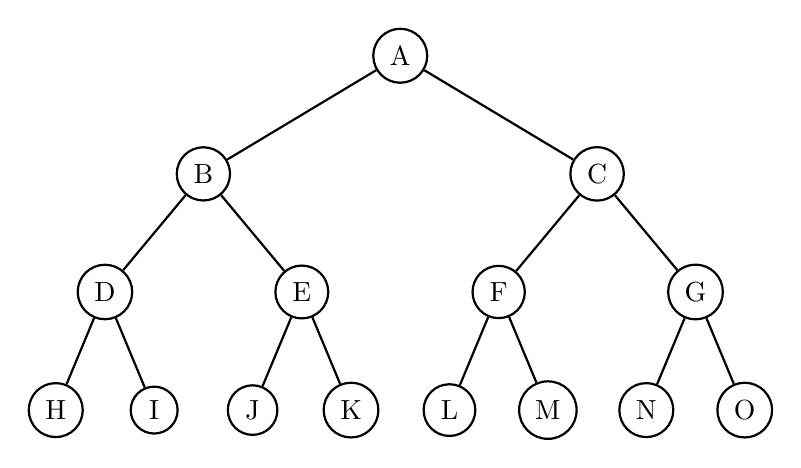
\begin{tikzpicture}[
  level distance=1.5 cm,
  level 1/.style={sibling distance=5cm},
  level 2/.style={sibling distance=2.5cm},
  level 3/.style={sibling distance=1.25cm}, thick]

  \node[circle,draw] {A}
	child {node[circle,draw]{B}
		child{node[circle,draw]{D}
			child{node[circle,draw]{H}}
			child{node[circle,draw]{I}}
		}
		child{node[circle,draw]{E}
			child{node[circle,draw]{J}}
			child{node[circle,draw]{K}}
		}
	}
	child{node[circle,draw]{C}
		child{node[circle,draw]{F}
			child{node[circle,draw]{L}}
			child{node[circle,draw]{M}}
		}
		child{node[circle,draw]{G}
			child{node[circle,draw]{N}}
			child{node[circle,draw]{O}}
		}
	};
\end{tikzpicture}
\caption{Example Graph 3}
\label{Bidirectional}
\end{figure}

Let A be an unweighted graph. This means that none of the edges of A has any value, or ``weight'' attached to it. How can we find the shortest path between two nodes?
One way would be to simply use a breadth-first search, stopping when we reach the
target node. The downside to this approach is that the algorithm would visit (at least)
every node on every level prior to the target node before it could end. Observe Graph 3 in Figure \ref{Bidirectional} above.
Let us use a simple BFS to search for O, starting with A as our root node.
We begin by searching through all of the neighbors of A, all of the neighbors of B
and C, and so on until we finally locate O. Using this method, we are forced to check
a total of $15$ nodes before our algorithm ends.

A better way to find the shortest path is to use a breadth-first search from
both A \emph{and} O. Thus, we find the shortest path using a pair of breadth-first searches originating from the root node and the target node, respectively.
We advance each BFS one node at a time, alternating until they meet, and then
construct the shortest path of nodes between our root and target.
Using the BFS algorithm from above, we start with A and locate its
least neighbor, B. Since we have not yet found O (or a connection to O) we visit G,
the first neighbor of O. Continuing in this pattern, we return to the neighbors
of A to visit C. Again, we return to our second search to visit the least neighbor of
G, which is also C. We have found our connection, so the algorithm ends. Note that when we used a breadth-first
search with only one root node, we visited $15$ nodes, but when we used a bidirectional BFS, we only had to visit $5$ nodes to find our path.

The speedup from doing a breadth-first search from both sides is especially evident in larger graphs, where each level
contains more nodes as we search away from our root. Indeed, a bidirectional search is one of the best ways to find shortest
paths in unweighted, undirected graphs. For weighted graphs there are many algorithms
that allow us to find the shortest path. For further information research Dijkstra's Algorithm, Johnson's algorithm, the Bellman--Ford algorithm, the Floyd--Warshall algorithm, and A* search algorithm.

\section*{Six Degrees of Kevin Bacon}
\begin{figure}[h]
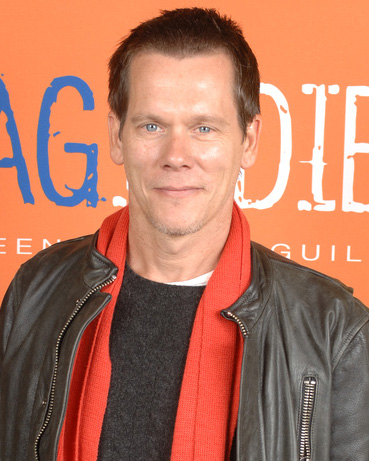
\includegraphics[scale = .4]{Kevin_Bacon.jpg}
\caption{Kevin Bacon.  Image source: Wikipedia.}
\end{figure}

The theory of ``the 6 Degrees of Separation'' suggests that each person in the world can be linked to any other person by 6 or less steps, or degrees, of acquaintanceship.
Similarly, the game ``the 6 Degrees of Kevin Bacon'' contends that every actor in the film industry can be linked to Kevin Bacon by 6 degrees or less. Kevin Bacon
is a prolific American actor whose film career spans over 30 years in a variety of genres. As such, he once reputably commented that he had either worked with everyone in
Hollywood or someone who has worked with them. The goal of the game, then, is to find the lowest Bacon number for each actor, a process demonstrated as follows:
\begin{enumerate}
\item Kevin Bacon has a Bacon number of $0$.
\item Actors that have been in a movie with Kevin Bacon have a Bacon number of $1$.
\item For all other actors $X$, if $n$ is the lowest Bacon number of any actor that $X$ has been in a film with, $X$ has a Bacon number of $n+1$.
\end{enumerate}

\begin{figure}[h]

\includegraphics[scale = .6]{Example}
\caption{Jeffrey Humphery was in \emph{End Game} with Cuba Gooding Jr., who was in \emph{A Few Good Men} with Kevin Bacon, so Jeffrey Humphrey has a Bacon Number of 2.  Image source: http://oracleofbacon.org/.}
\end{figure}

We can define a graph in the same way: where each actor is a node and there is an edge between any two nodes if their actors were in a movie together. From this structure we can find
the shortest path between any actor and Kevin Bacon by using any of the algorithms listed above. Of course, this game is not limited to Kevin Bacon; we could use any actor as our ``root actor.''
In fact, ``the Six Degrees of Separation'' can be applied to many different fields. Its most famous application is known as the Erdos numbers: how far away is a person
 from publishing a paper (rather than starring in a movie) with the prolific mathematician Paul Erdos?

\section*{NetworkX}
For this lab, we are going to use a network library called NetworkX. NetworkX is a useful Python package that allows us to create and manipulate large, complex networks.
When considering efficiency, however, it is important to note that because NetworkX uses Python objects to represent its graphs internally, graphs with many nodes will
use a large chunk of memory. (Other network libraries, such as igraph, are written in C++ and may therefore significantly reduce the overhead of storing such a graph.)
To make an undirected graph in NetworkX, we simply code the following:

\begin{lstlisting}
import networkx as nx
G = nx.Graph()
\end{lstlisting}

As an example, we will create a NetworkX graph that links the ingredients of
delicious americanized Italian foods together. We first want to add the ingredients as nodes
to our graph. To add nodes we can use either the \li{add_node(x)} method, where $x$
is the node we want to add, or the \li{add_nodes_from()} method, to
add multiple nodes at once.

\begin{lstlisting}
import networkx as nx
G = nx.Graph()

G.add_node('dough')
PizzaIngredients = ['dough', 'mozzarella cheese', 'tomato sauce', 'ham', 'pineapple']
G.add_nodes_from(PizzaIngredients)
\end{lstlisting}
Note that even though we added \li{'dough'} twice, the graph will only store this node once. NetworkX also comes with \li{has_node(x)} and \li{has_edge(x,y)} methods that will tell
us if a node $x$ or an edge $(x,y)$ has already been added.

Now we want to connect our pizza ingredients together. Adding an edge is simple; we just use the \li{add_edge(x,y)} method, where $x$ and $y$ are previously added nodes.
Again, we can also add multiple edges using the \li{add_edges_from()} method.
However, these edges must be provided as 2-tuples \li{(x,y)}, so we use the
itertools module to create a list of the edges we want to add. It might be wise
to review previous labs and the python documentation for this module as you implement
NetworkX graphs.

\begin{lstlisting}
from itertools import permutations
Pizza = permutations(PizzaIngredients, 2)
G.add_edges_from(Pizza)
\end{lstlisting}
If we add an edge between two non-existent nodes, the missing nodes will also be added to the graph. Let's add the ingredients for lasagna to the graph using only the \li{add_edges_from} method.
\begin{lstlisting}
LasagnaIngredients = ['lasagna noodles', 'sausage', 'mozzarella cheese', 'cottage cheese', 'tomato sauce', 'egg', 'parsley']
Lasagna = permutations(LasagnaIngredients, 2)
G.add_edges_from(Lasagna)
\end{lstlisting}
We can also remove nodes using the methods \li{remove_node(x)} and \li{remove_nodes_from()}.
Let's say, for example, that we are vegetarians and want to remove the
sausage and ham from our graph. Then, we simply run the following code:
\begin{lstlisting}
G.remove_nodes_from(['sausage', 'ham'])
\end{lstlisting}

Sometimes, with smaller graphs, it can be useful to visualize how nodes are linked together. However, the overhead associated with displaying larger graphs makes this unwise for extensive data sets.
For our example, though, it makes it easy to see the connections between our lasagna and pizza ingredients:

\begin{lstlisting}
# MatPlotLib is a standard Python plotting library; it allows you to plot
# and display your 2D graph.
import matplotlib.pyplot as plt
# Allows you to draw a simple diagram of the nodes and their connecting edges.
nx.draw(G)
# Displays your graph.
plt.show()
\end{lstlisting}


\begin{problem}
The data file, \texttt{movieData.txt}, contains the entire casts of movies made over the course of several years. It is a delimited file with each field delimited by the `/' character. Write a method that will implement the following:
\begin{itemize}
\item Open the file.
\item Generate a NetworkX graph, with the actors as nodes and with edges connecting all of the actors within the same movie to one another. Do not include movie titles as nodes.
\item Return your constructed NetworkX graph (note that, because of the large amount of data, you \textbf{should not} attempt to display this graph).
\end{itemize}
\emph{Helpful Hints:}
\begin{itemize}
\item For later solutions, it might be beneficial to also construct a map from the actors to the movies they appeared in.
\item For certain machine types, take care to open your file using universal newline support. See previous labs for further information.
\end{itemize}
\end{problem}

For a graph, G, the \li{shortest_path(G, x, y)} function in NetworkX outputs
the shortest path from $x$ to $y$ as a list. If more than one such path exists,
it will simply return the first of the shortest paths that it finds. In an
unweighted graph, this method finds the shortest path using a bidirectional search,
a process outlined earlier in this chapter. However, if no path exists between nodes
$x$ and $y$ then NetworkX will raise an exception. If we don't specify a
target, then the function will find the shortest paths between our root,
$x$, and every other node in the network.  It will return the results as a dictionary.


We can find the length of the shortest path using the \li{shortest_path_length(G, x, y)}
function. Again, the target node for this function is optional; if we only
specify the graph and the root node, \li{shortest_path_length()} will return a dictionary
with all \emph{connecting} nodes as keys. When we don't provide a target, if no path exists between the root
and another node then NetworkX will simply omit that node from the dictionary (rather than raise an exception).

\begin{problem}
Find the shortest path between Kevin Bacon and Liam Neeson. Then find the shortest path from Kevin Bacon to Imran Zahid. Write a function that will accept two actors and output
the path between them, along with the movies in between that connect each step of the path. Output the paths from Kevin Bacon to Liam Neeson and Imran Zahid along with the connecting movies.
\end{problem}

\begin{problem}
Find the average Bacon number for the dataset. Then find the number of actors
associated with each Bacon number and the number of actors that have no connection
 to Kevin Bacon at all (we would say these people have a Bacon number of infinity).
\end{problem}

